%!TEX root = ../book.tex
\section{Forward Kinematics}\label{sec:kinematics:fwd}

Now that we have introduced the notion of local coordinate frames, we are interested in calculating the pose and speed of these coordinate frames as a function of the robot's actuators and joint configuration.
That is, we are interested in computing a function $f$ that allows us to map a joint configuration to its corresponding end-effector pose:
\begin{equation}\label{eq:kinematics:forward}
r=f(q)\ , \qquad f : \mathbb{R}^n \rightarrow \mathbb{R}^m \ ,
\end{equation}
where $r$ is the task-space (end-effector) configuration and $q$ is the joint-space configuration.
It is important to remember that the choice of $q$ and $r$ (and, consequently, the complexity of $f$) depends on your specific robot platform and the specific task you are investigating.
$q$ generally corresponds to the number of actuators/joint that you can control on your robot; it is of size $n$, where $n$ is the number of degrees of freedom in joint space (see also \cref{sec:dof}).
Conversely, $r$ depends on the task and its dimensionality is $m$, where $m$ is the number of DoFs in task space.
% (e.g. a sequence of joint angles in case of a manipulator with revolute joints \td{we have not talked about revolute joints yet, remember to fix this}).

In the following, we will focus on the problem of computing the forward kinematics mapping $f$ for a variety of robot arms.
While it is always possible to compute the forward kinematics \textsl{analytically} (i.e. by inspecting the arm mechanism and the relationship between joint and task configuration, see \cref{sec:kinematics:fwk:arm}), in \cref{sec:kinematics:fwk:dh} we will introduce a scalable, \textsl{geometric} technique to compute forward kinematics with more complex arms composed of many Degrees of Freedom.
% number of selected but diverse mechanisms.
% We will first consider simple mechanisms where we can determine the relationship between actuators and the pose of various frames on the robot both in the position and speed domain.
% We will then consider the special class of non-holonomous mechanisms using a series of wheeled robots, for which the forward kinematics can only be calculated in the speed domain.

\subsection{Forward Kinematics of a simple robot arm}\label{sec:kinematics:fwk:arm}

\begin{figure}[!htb]%{L}{0.3\textwidth}
    \centering
    % 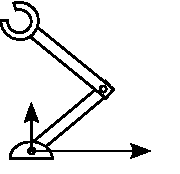
\includegraphics[width=0.27\textwidth]{figs/fwk2dofarm}
    \def\svgwidth{0.4\textwidth}
    \import{./figs/kinematics/}{fwk2dofarm.pdf_tex}
    \caption{A simple 2-DOF arm.}\label{fig:fwk2dofarm}
\end{figure}

Consider the robot arm in \cref{fig:fwk2dofarm}; it is mounted to a table, and is composed of two links and two joints. Let the length of the first link be $l_1$ and the length of the second link be $l_2$. You could specify the position of the link closer to the table by the angle $\alpha$ and the angle of the second link relative to the first link using the angle $\beta$.
Therefore, in this case $q = [\alpha, \beta]^T$.
Our goal is to calculate the position $[x, y]^T$ and orientation $\theta$ of the end-effector; consequently, $f$ will map to $r = [x, y, \theta]^T$.

Let's now calculate the position $P_1 = (x_1, y_1)$ of the joint between the first and the second link using simple trigonometry:
%
\begin{eqnarray}\label{eq:cosxl1}
x_1 &=&l_1 \cos \alpha \nonumber \\
y_1 &=&l_1 \sin \alpha
\end{eqnarray}
%
Similarly, the position of the end-effector $P_2 = (x_2, y_2)$ is given by:
%
\begin{eqnarray}
x_2&=&x_1 + l_2 \cos(\alpha+\beta) \nonumber \\
y_2&=&y_1 + l_2 \sin(\alpha+\beta)
\end{eqnarray}
%
For what concerns the orientation of the arm's end-effector $\theta$, we know it is just the sum of $\alpha+\beta$.
Altogether, the configuration $r$ of the end-effector is given by:
%
\begin{eqnarray}\label{eq:fwk2dofarm}
x&=&l_1 \cos \alpha + l_2 \cos(\alpha+\beta) \nonumber \\
y&=&l_1 \sin \alpha + l_2 \sin(\alpha+\beta) \\
\theta&=& \alpha + \beta \nonumber
\end{eqnarray}
%
The above equations represent \textsl{the forward kinematic equations} of the robot---as they relate its control parameters $ \alpha$ and $\beta$ (also known as joint configuration) to the pose of its end-effector in the local coordinate system spanned by $x$ and $ y$ with the origin at the robot's base.
Note that both $\alpha$ and $\beta$ shown in the figure are positive: both links rotate around the $z-$axis. Using the right-hand rule, the direction of positive angles is defined to be counter-clockwise.

The \textsl{configuration space}\index{Configuration space}\index{C-Space (Configuration space)} of the robot---i.e. the set of angles each actuator can be set to---is given by $ 0 < \alpha < \pi $ as it is not supposed to run into the table, and $ -\pi < \beta < \pi$.
The configuration space is given with respect to the robot's joints and allows us to use the forward kinematics equations to calculate the \textsl{workspace}\index{Workspace} of the robot, i.e. the physical space it can move to.
This terminology will be identical for mobile robots. An example of configuration and workspace for both a manipulator and a mobile robot is shown in \cref{fig:holonomy}.

% As shown in \cref{fig:fwk2dofarm}, the orientation of the arm's end-effector is given by $\alpha+\beta$.
We can now write down  a transformation that includes a rotation around the z-axis:
\begin{equation}
\label{eq:2armtrans}
f(q) = \left[\begin{array}{cccc}c_{\alpha\beta} & \ -s_{\alpha\beta} & \  0 & \ c_{\alpha\beta}l_2+c_\alpha l_1\\
                        s_{\alpha\beta} & \ c_{\alpha\beta} & \ 0 & \ s_{\alpha\beta}l_2+s_\alpha l_1\\
                                                0 & \ 0 & \ 1 & \ 0\\
                                                0 & \ 0 & \ 0 & \ 1\end{array}\right]
\end{equation}
The notation $s_{\alpha\beta}$ and $c_{\alpha\beta}$ are shorthand for $sin(\alpha+\beta)$ and $cos(\alpha+\beta)$, respectively.
%
This transformation now allows us to transform from the robot's base to the robot's end-effector configuration $r = [x, y, \theta]^T$ as a function of the joint configuration $q = [\alpha, \beta]^T$.
This transformation will be helpful if we want to calculate suitable joint angles in order to reach a certain pose (i.e., inverse kinematics) or if we want to convert measurements taken relative to the end-effector back into the base's coordinate system (e.g., when we have sensors mounted on the end effector whose output needs to be mapped back to the world reference frame).


\subsection{The Denavit-Hartenberg notation}\label{sec:kinematics:fwk:dh}

So far, we have considered the forward kinematics of a simple arm and derived relationships between actuator parameters and end-effector positions using basic trigonometry.
In the case of multi-link arms (which is the vast majority of robot manipulators in existence), the approach detailed in \cref{sec:kinematics:fwk:arm} is difficult to scale, and alternative solutions are needed.
Interestingly, we can think of the forward kinematics as a chain of homogeneous transformations with respect to a coordinate system mounted at the base of a manipulator or a fixed position in the room.
Deriving these transformations can be confusing and can be facilitated by following a ``recipe'' such as the one conceived by Denavit and Hartenberg in $1955$ (see \cite{hartenberg1955kinematic} and \cite{craig2009introduction}).
The so-called Denavit-Hartenberg (DH)\index{Denavit-Hartenberg parameters} representation has since evolved as a \textsl{de-facto} standard.

A manipulator consists of a series of typically rigid links that are connected by joints.
In the vast majority of cases, a joint can either be revolute (i.e. change its angle/orientation) or prismatic (i.e. change its length).
Knowing the robot's kinematic properties (e.g. the length of all rigid links, similarly to $l_1$ and $l_2$ in \cref{fig:fwk2dofarm}), the pose of its end-effector is fully described by its joint configuration (angle for revolute joints, length for prismatic joints).

%In industrial manipulators, the number of joints is usually equal to the degrees of freedom of the manipulator. As most manipulators are holonomic, the forward kinematics allow you---unlike on non-holonomic wheeled platforms---to directly relate absolute positions of joints with absolute positions in Cartesian space. It is also possible to derive equations that relate the speed of the joints to speed in Cartesian space. Like for wheeled platforms, this can be achieved via a Jacobian matrix.  At certain positions, the mapping provided by the Jacobian is not invertible, i.e., some velocities in Cartesian space are unachievable. These points are called singularities.

\screencast{http://youtu.be/rA9tm0gTln8}{denavithartenberg}

\begin{figure}[!t]
    \centering
    % 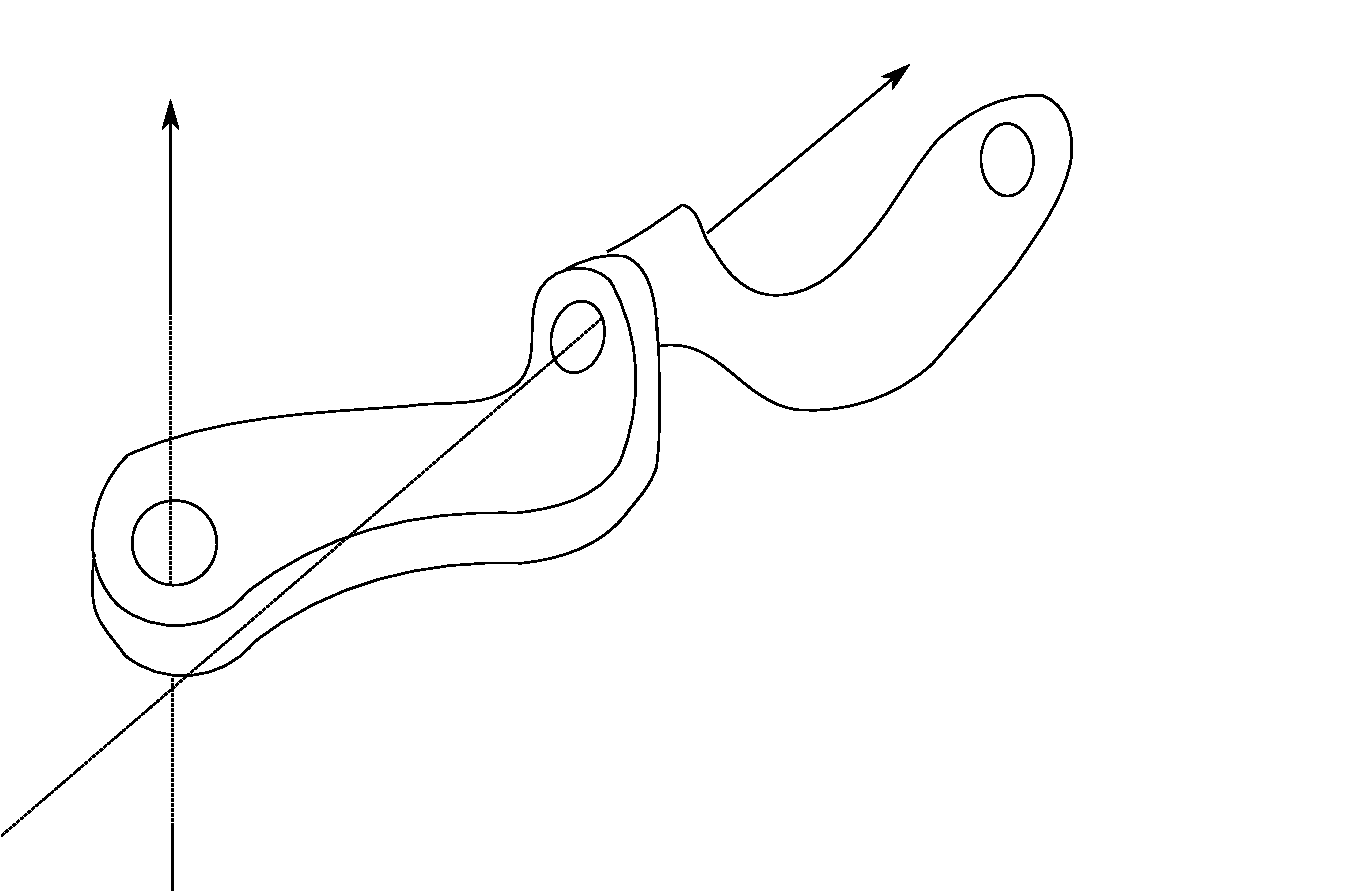
\includegraphics[width=\textwidth]{figs/denavit-hartenberg.png}
    \def\svgwidth{\textwidth}
    \import{./figs/kinematics/}{denavit-hartenberg.pdf_tex}
    \caption{Example of selected Denavit-Hartenberg parameters for three sequential revolute joints. The z-axes of joint $i$ and $i+1$ are parallel, which results in $\alpha_i = 0$.}
    \label{fig:denavit}
\end{figure}

In order to use the DH convention, we first need to define a coordinate system at each joint. With reference to \cref{fig:denavit}, we choose the $z-$axis to be the axis of rotation for a revolute joint and the axis of translation for a prismatic joint.
We can now find the common normal between the $z-$axes of two subsequent joints, i.e. a line that is orthogonal to each $z-$axis and intersects both.
With the direction of the $x-$axis at the base arbitrary, subsequent $x-$axes are chosen such that they lie on the common normal shared between two joints.
Whereas the direction of the $z-$axis is given by the positive direction of rotation (right-hand rule), the $x-$axis points away from the previous joint.
This allows defining the $y-$axis using the right-hand rule.
Note that these rules, in particular the requirement that $x$-axes lie along the commom normal, might result in coordinate systems with their origins outside the joint: this is not relevant as the kinematics of a manipulator is a mathematical representation that needs to represent the geometric and kinematic properties of the robot, and does not need to bear any physical correspondence.
%
The transformation between two joints is then fully described by the following four parameters:
\begin{enumerate}
\item The length $r$ (sometimes, $a$ is used) of the common normal between the $z$-axes of two joints $i$ and $i-1$ (link length).
\item The angle $ \alpha$ between the z-axes of the two joints with respect to the common normal (link twist), i.e. the angle between the old and the new $z$-axis, measured about the common normal.
\item The distance $d$ between the joint axes (link offset), i.e. the offset along the previous $z$-axis to the common normal.
\item The rotation $ \theta$ around the common axis along which the link offset is measured (joint angle), i.e. the angle from the old $x$-axis to the new $x$-axis, about the previous $z$-axis.
\end{enumerate}

Two of the above D-H parameters describe the link between the joints, and the other two describe the link's connection to a neighboring link.
Depending on the link/joint type, these numbers are fixed by the specific mechanical instance of the robot or can be controlled.
For example, in a revolute joint $ \theta$ is the varying joint angle, while all other quantities are fixed.  Similarly, for a prismatic joint $d$ is the joint variable. An example of two revolute joints is shown in \cref{fig:denavit}.

The final coordinate transform from one link ($i-1$) to another ($i$) can now be constructed by concatenating the four steps above, which are nothing but a series of rotations and translations, one for each DH parameter:
%
\begin{equation}\label{eq:kinematics:dh:composition}
_{n-1}^nT=T_z'(d_n) R_z'(\theta_n) T_x(r_n)  R_x(\alpha_n)
\end{equation}
with
\begin{equation}
T_z'(d_n)=
\left[ \arraycolsep=2pt%\def\arraystretch{2.2}
\begin{array}{ccc|c}
1 & 0 & 0 & 0\\
0 & 1 & 0 & 0\\
0 & 0 & 1 & d_n\\
\hline
0 & 0 & 0 & 1
\end{array}
\right]
\enskip
R_z'(\theta_n)=\left[ \arraycolsep=2pt%\def\arraystretch{2.2}
\begin{array}{ccc|c}
\cos\theta_n & -\sin\theta_n & 0 & 0\\
\sin\theta_n & \cos\theta_n & 0 & 0\\
0 & 0 & 1 & 0\\
\hline
0 & 0 & 0 & 1
\end{array}
\right]
\end{equation}
and
\begin{equation}
T_x(r_n)=
\left[ \arraycolsep=2pt%\def\arraystretch{2.2}
\begin{array}{ccc|c}
1 & 0 & 0 & r_n\\
0 & 1 & 0 & 0\\
0 & 0 & 1 & 0\\
\hline
0 & 0 & 0 & 1
\end{array}
\right]
\enskip
R_x(\alpha_n)=\left[ \arraycolsep=2pt%\def\arraystretch{2.2}
\begin{array}{ccc|c}
1 & 0 & 0 & 0\\
0 & \cos\alpha_n & -\sin\alpha_n & 0\\
0 & \sin\alpha_n & \cos\alpha_n & 0\\
\hline
0 & 0 & 0 & 1
\end{array}
\right]
\end{equation}
%
These are a translation of $d_n$ along the previous z-axis ($T_z'(d_n)$), a rotation of $\theta_n$ about the previous z-axis ($R_z'(\theta_n)$), a translation of $r_n$ along the new $x$-axis ($T_x(r_n)$)and a rotation of $\alpha_n$ around the new $x$-axis ($R_x(\alpha_n)$).
%
By replacing each element in \cref{eq:kinematics:dh:composition}, the following matrix is created:
\begin{eqnarray}
_{n-1}^nT&=
\left[ \arraycolsep=2pt%\def\arraystretch{2.2}
\begin{array}{ccc|c}
\cos \theta_n & -\sin \theta_n \cos\alpha_n & \sin\theta_n \sin\alpha_n & r_n \cos\theta_n\\
\sin \theta_n & \cos\theta_n \cos\alpha_n & -\cos\theta_n\sin\alpha_n & r_n \sin\theta_n\\
0 & \sin\alpha_n & \cos\alpha_n & d_n \nonumber \\
\hline
0 & 0 & 0 & 1
\end{array}
\right]\\
&=
\left[ \arraycolsep=2pt%\def\arraystretch{2.2}
\begin{array}{c|c}
R & t\\
\hline
0 \quad 0 \quad 0 & 1
\end{array}
\right]
\end{eqnarray}
where $R$ is the $3\times3$ rotation matrix and $t$ is the $3\times1$ translation vector.

Like for any homogeneous transform, the inverse $_{n-1}^nT^{-1}n$ is given by
\begin{equation}
^{n-1}_nT=\left[ \arraycolsep=2pt%\def\arraystretch{2.2}
\begin{array}{c|c}
R^{-1} & -R^{-1}T\\
\hline
0 \quad 0 \quad 0 \quad 1
\end{array}
\right]
\end{equation}
with the inverse of $R$ simply being its transpose, $R^{-1}=R^T$.

Similar to the concatenation of transformations detailed in \cref{sec:kinematics:coordsystems:concatenation}, $_{n-1}^nT$ in \cref{eq:kinematics:dh:composition} can be concatenated with the other transformation matrices relative to the remaining links in order to compute a the full kinematics of the robot arm from the base reference frame up to the end-effector.
% \td{Nikolaus, should we add half a page of text plus a figure to describe this further? I feel they are left hanging without it}
